% OCR draft from PDF pages 151-152. Needs cleanup and verification.
\chapter{A Multiprocessor System Model}
\label{chap:multiprocessor-system}

\section{Introduction}
\label{sec:mp-introduction}

In earlier chapters, we discussed two smpl simulation models: a simple
single-server queueing system model and a two-class queueing network model.
In this chapter, we'll look at another example: a model of memory and bus
contention in a multiprocessor system. This example presents some new
modeling problems and further illustrates the use of smpl. We'll begin by
developing an analytic model of the system, and then develop a simulation
model to check the analytic results. After cross-verifying analytic and
simulation results, we'll consider ways of extending the simulation model to
eliminate some of the assumptions used in the analytic approach.

\section{The Multiprocessor System}
\label{sec:mp-system}

The system we'll be studying is diagrammed in Figure 5.1. It comprises $N$
processors and $M$ global memory modules (or, simply, memories) interconnected
by $B$ buses so that every processor can access every memory. Transfers between
processors and memories take place in fixed-size units equal to the bus width,
so that each transfer requires one bus cycle. The system is synchronous: all
memory requests are initiated at the same point in a cycle.

We'll assume -- at least for now -- that the $N$ processors are physically and
functionally identical. Each processor has its own local memory, which may be a
cache or may take the form of data registers and an instruction buffer. When
executing, a processor issues an instruction fetch or an operand fetch or store
request in every machine cycle. This request is satisfied in the processor's
local memory with probability $h$ and requires access to (global) memory with
probability $p = 1 - h$. $h$ is called the hit ratio and $p$ is called the miss
ratio. Memory request processing takes place as follows.

\begin{figure}[ht]
\centering
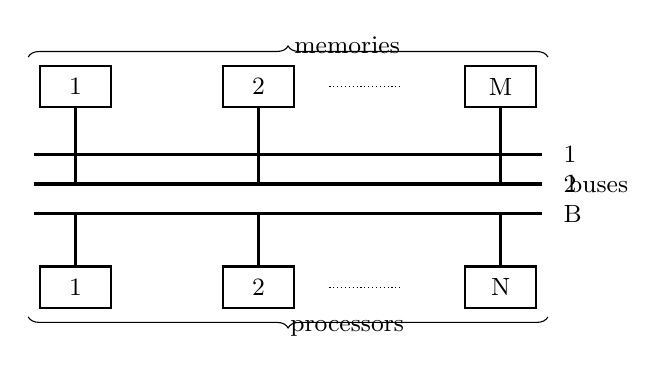
\begin{tikzpicture}[x=0.75cm,y=0.75cm]
  \draw[line width=0.9pt] (1,6.5) rectangle (2.2,7.2) node[midway]{\small 1};
  \draw[line width=0.9pt] (4.1,6.5) rectangle (5.3,7.2) node[midway]{\small 2};
  \draw[line width=0.9pt] (8.2,6.5) rectangle (9.4,7.2) node[midway]{\small M};
  \node at (6.2,7.55) {\small memories};
  \draw[decorate,decoration={brace,amplitude=4pt}] (0.8,7.35) -- (9.6,7.35);

  \draw[line width=1.1pt] (0.9,5.7) -- (9.5,5.7);
  \draw[line width=1.1pt] (0.9,5.2) -- (9.5,5.2);
  \draw[line width=1.1pt] (0.9,4.7) -- (9.5,4.7);
  \node[right] at (9.7,5.7) {\small 1};
  \node[right] at (9.7,5.2) {\small 2};
  \node[right] at (9.7,4.7) {\small B};
  \node at (10.45,5.2) {\small buses};

  \draw[line width=0.9pt] (1,3.1) rectangle (2.2,3.8) node[midway]{\small 1};
  \draw[line width=0.9pt] (4.1,3.1) rectangle (5.3,3.8) node[midway]{\small 2};
  \draw[line width=0.9pt] (8.2,3.1) rectangle (9.4,3.8) node[midway]{\small N};
  \node at (6.2,2.75) {\small processors};
  \draw[decorate,decoration={brace,mirror,amplitude=4pt}] (0.8,2.95) -- (9.6,2.95);

  \foreach \x in {1.6,4.7,8.8} {
    \draw[line width=0.9pt] (\x,6.5) -- (\x,5.2);
    \draw[line width=0.9pt] (\x,4.7) -- (\x,3.8);
  }
  \draw[densely dotted] (5.9,6.85) -- (7.1,6.85);
  \draw[densely dotted] (5.9,3.45) -- (7.1,3.45);
\end{tikzpicture}
\caption{Multiprocessor System Elements}
\end{figure}

\begin{enumerate}
\item A processor initiates a memory request at the start of a machine cycle
  and simultaneously suspends execution. Multiple requests for the same module
  are resolved by an arbitration mechanism. We'll assume that this mechanism
  tries to provide fair service via a cyclical scan of processors for requests,
  with the scan starting point being advanced on each new scan.
\item If a request is successful, the module is reserved for the processor;
  otherwise, the request is reissued at the start of the next cycle. From the
  set of up to $M$ successful requests, a second arbitration mechanism selects
  up to $B$ requests and reserves buses for these requests. We'll assume this is
  done in the same order in which modules were reserved. If a request is
  unsuccessful in obtaining a bus, the module is released and the request
  reissued at the start of the next cycle.
\item Next, for a successful request, the address and data (if the request is
  a store) are transmitted over the bus to memory; if the request is a fetch,
  data is returned over the bus at the end of the cycle.
\item When the bus cycle ends, processors whose requests were successfully
  completed are returned to execution, and the buses and modules reserved by
  these requests are released. Unsuccessful requests are reissued, together
  with new requests, at the start of the next cycle.
\end{enumerate}

Our objective is to determine how processor performance is affected by
contention for memory modules and buses.

This system, in various forms, has received a great deal of attention over
the years. When the number of buses is equal to the number of memories
($B = M$), the interconnection between processors and memories is equivalent to
a crossbar network, and performance is affected only by memory contention.
Most of the early analysis work focused on this problem; most recent work
encompasses systems with $B < M$ and considers both bus and memory contention.

\section{An Approximate Analytic Model}
\label{sec:mp-analytic-model}

The analytic model developed here is based on Mudge et al.\ [1984]; the
references in that paper provide a good starting point for surveying work in
this area. There are several measures of performance of interest; the one
considered first is system bandwidth, $BW$. This is the overall transfer rate
between processors and memory, in transfers per unit time. Since transfer time
is one cycle, overall bus utilization is (numerically, though not
dimensionally) equal to $BW$, and $BW$ is sometimes defined as the average
number of busy buses.

The miss ratio $p$ was defined as the probability that a processor issues a
(global) memory request in a given cycle. If we assume that the probability of
issuing a request in one cycle is the same as, and independent of, the
probability of issuing a request in any other cycle, then a processor's
execution interval corresponds to a sequence of Bernoulli trials. Execution
intervals therefore have a geometric distribution with mean
$x = (1-p)/p$ and variance $\sigma_x^2 = (1-p)/p^2$. We also assume that memory
requests are independently and uniformly distributed across memories.

Looking first at cycles with no reissued requests from the preceding cycle, the
probability that processor $i$ requests memory $j$ is $p/M$, and the
probability that none of the $N$ processors requests memory $j$ is
$(1 - p/M)^N$. Therefore the probability $q$ that there is at least one request
for memory $j$ is

\begin{equation}
q = 1 - (1 - p/M)^N
\label{eq:mp-q-p}
\end{equation}

Assuming request probabilities are identical and independent, the probability
$f_i$ that exactly $i$ of $M$ memories have requests is binomial:

\begin{equation}
f_i = \binom{M}{i} q^i (1-q)^{M-i}
\label{eq:mp-fi}
\end{equation}

The expected number of distinct memories requested in a cycle is $qM$. While up
to $qM$ requests may be presented to bus arbitration in a cycle, no more than
$B$ requests can be granted. The expected number of bus requests granted in a
cycle (equal numerically to bandwidth) is

\begin{equation}
BW = B\sum_{i=B}^{M} f_i + \sum_{i=1}^{B-1} i f_i
\label{eq:mp-bw}
\end{equation}

The bandwidth estimate from (\ref{eq:mp-q-p})--(\ref{eq:mp-bw}) applies only to
cycles in which no requests are reissued; in that case the average request rate
per processor is the miss rate $p$, and overall request rate is $Np$. In the
general case, considering all cycles, the per-processor request rate $r$ is
greater than $p$ (because it includes both initial and reissued requests). An
exact analysis is difficult; however, if we can estimate $r$, we can use it in
place of $p$ in (\ref{eq:mp-q-p}) to obtain an improved estimate of $BW$.

Now consider the processor inter-request interval between successful request
completions. Its mean overall length is $T$, and can be divided into three
parts: an execution interval of mean length $x = (1-p)/p$, a delay interval of
mean length $b$, and a one-cycle transfer time for the accepted request. The
single-processor request rate (counting blocked and accepted requests) is

\begin{figure}[ht]
\centering
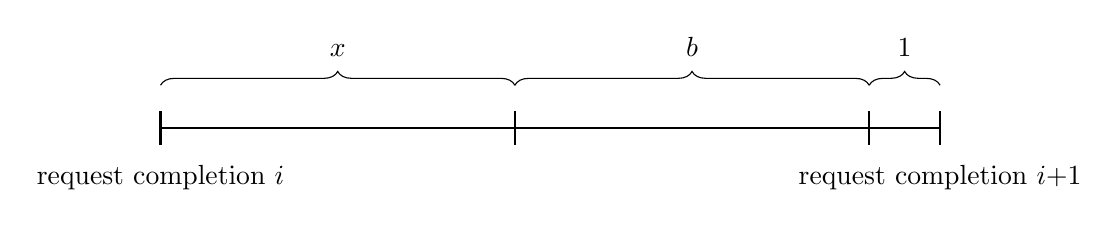
\begin{tikzpicture}[x=0.9cm,y=0.9cm]
  % Processor inter-request interval: execution x, blocked delay b, transfer 1.
  \draw[line width=0.9pt] (0,0) -- (11,0);
  \foreach \x in {0,5,10,11} {
    \draw[line width=0.9pt] (\x,0.24) -- (\x,-0.24);
  }
  \draw[decorate,decoration={brace,amplitude=5pt}] (0,0.6) -- (5,0.6)
    node[midway,above=7pt] {$x$};
  \draw[decorate,decoration={brace,amplitude=5pt}] (5,0.6) -- (10,0.6)
    node[midway,above=7pt] {$b$};
  \draw[decorate,decoration={brace,amplitude=5pt}] (10,0.6) -- (11,0.6)
    node[midway,above=7pt] {$1$};
  \node[below=10pt] at (0,0) {request completion $i$};
  \node[below=10pt] at (11,0) {request completion $i{+}1$};
\end{tikzpicture}
\caption{Processor Inter-Request Interval Timing}
\label{fig:ch5-inter-request-interval}
\end{figure}

\begin{equation}
r = (b+1)/T = (b+1)/(x+b+1)
\label{eq:mp-r}
\end{equation}

or

\begin{equation}
r = \left[1 + x/(b+1)\right]^{-1}
\label{eq:mp-r-alt}
\end{equation}

The per-processor request completion rate is $BW/N$, so $T = N/BW$, and
$b+1 = rT = Nr/BW$. Substituting in (\ref{eq:mp-r-alt}),

\begin{equation}
r = \left[1 + xBW/(Nr)\right]^{-1}
\label{eq:mp-r-fp}
\end{equation}

which defines $r$ as a fixed-point function of itself and can be solved
iteratively:

\begin{enumerate}
\item Use (\ref{eq:mp-q-p})--(\ref{eq:mp-bw}) to compute an initial bandwidth
  estimate $BW_1$. Define $r_1 = p$.
\item Compute an improved estimate of $r$ from
  \begin{equation}
  r_i = \left[1 + xBW_{i-1}/(Nr_{i-1})\right]^{-1}
  \label{eq:mp-ri}
  \end{equation}
\item Compute
  \begin{equation}
  q = 1 - (1-r_i/M)^N
  \label{eq:mp-q-r}
  \end{equation}
  and use (\ref{eq:mp-fi}) and (\ref{eq:mp-bw}) to compute a new estimate
  $BW_i$.
\item If $|BW_i - BW_{i-1}| < \epsilon$, where $\epsilon$ depends on desired
  accuracy, terminate; otherwise return to step 2.
\end{enumerate}

A C implementation with $\epsilon=0.005$ is shown in Figure~\ref{fig:ch5-bw-code}.

\begin{figure}[ht]
\centering
\begin{minipage}{0.86\textwidth}
\begin{verbatim}
real BW(real p, int B, int M, int N)
{
  real r = p, bw_prev = 0.0, bw = 0.0;
  while (1) {
    real q = 1.0 - pow(1.0 - r/M, N);
    bw = 0.0;
    for (int i = 1; i <= M; ++i) {
      real fi = comb(M,i) * pow(q,i) * pow(1-q, M-i);
      bw += (i < B) ? i*fi : B*fi;
    }
    if (fabs(bw - bw_prev) < 0.005) break;
    r = 1.0 / (1.0 + ((1-p)/p) * bw / (N*r));
    bw_prev = bw;
  }
  return bw;
}
\end{verbatim}
\end{minipage}
\caption{Bandwidth Computation Algorithm}
\label{fig:ch5-bw-code}
\end{figure}

Timing relationships and operational laws give other measures. Average
utilization of a single bus, memory module, and processor are respectively
$U_B = BW/B$, $U_M = BW/M$, and $U_P = xBW/N$. Average waiting time per request
is $b$, where from $T=N/BW$ and $x+1=1/p$:

\begin{equation}
b = (N/BW) - (1/p)
\label{eq:mp-b}
\end{equation}

Mean number of blocked requests per processor $L_b$ follows from Little's Law:

\begin{equation}
L_b = bBW/N
\label{eq:mp-lb}
\end{equation}

so

\begin{equation}
L_b = 1 - BW/(Np)
\label{eq:mp-lb-alt}
\end{equation}

For system throughput, if each task requires an average of $n$ execution
intervals, service time per task is $nx$. Throughput is $N[U_P/(nx)]$ tasks per
unit time. A normalized throughput $\eta$ with $nx=1$ is

\begin{equation}
\eta = N U_P = BW\left[(1/p)-1\right]
\label{eq:mp-eta}
\end{equation}

This bandwidth analysis is approximate, in part because
(\ref{eq:mp-q-p})--(\ref{eq:mp-fi}) assume independent memory request
probabilities. In the actual system, a blocked request for module $j$ is
reissued to $j$, so request probability for module $j$ in cycle $n$ is not
independent of cycle $n-1$. The next section develops a simulation model for
verification and evaluation of this assumption.

\section{Verifying the Analytic Model}
\label{sec:mp-verify}

The simulation model used for analytic verification depends on objective. Here
the objective is to verify that the analytic model adequately represents system
behavior, so the simulation model reflects system structure. A smpl model for
this purpose (called \texttt{bws1} in the book) is given in Figure 5.4.

\begin{figure}[ht]
\centering
\begin{minipage}{0.86\textwidth}
\begin{verbatim}
/* model bws1: synchronous multiprocessor */
init_model(p, N, M, B) {
  for (j=1; j<=M; j++) module[j] = facility("module", 1);
  bus = facility("bus", B);
  for (n=1; n<=N; n++) schedule(BEGIN_CYCLE, 0.0, n);
}

begin_cycle(n) {
  if (req[n] != 0) return;
  if (drand() < p) {
    req[n] = randint(1, M);
    schedule(REQ_MODULE, 0.0, n);
  } else {
    schedule(BEGIN_CYCLE, 1.0, n);
  }
}

req_module(n) {
  if (!busy(module[req[n]]) && !busy(bus)) {
    reserve(module[req[n]]); reserve(bus);
    schedule(END_CYCLE, 1.0, n);
  } else {
    schedule(REQ_MODULE, 1.0, n);   /* reissue */
  }
}

end_cycle(n) {
  release(module[req[n]]); release(bus);
  req[n] = 0; schedule(BEGIN_CYCLE, 0.0, n);
}
\end{verbatim}
\end{minipage}
\caption{Multiprocessor Simulation Model \texttt{bws1}}
\label{fig:ch5-bws1}
\end{figure}

In this model, memory modules and buses are smpl facilities, while processors
are represented as tokens. Global declarations define miss rate $p$, number of
processors $N$, memories $M$, and buses $B$ (named \texttt{nB} to avoid
conflict with \texttt{B()} in smpl), with facility descriptors
\texttt{module[]} and \texttt{bus}. \texttt{treg[n]} records next memory request
issue time for processor $n$, \texttt{req[n]} records requested module number,
and \texttt{tn} is the earliest request time. Initialization calls
\texttt{smpl()}, declares facilities, computes each initial access time, and
schedules the first event.

The continuation of the model appears in Figure~5.4 (continued): event 1
(\texttt{begin cycle()}) scans processors for requests at time \texttt{tn};
event 2 (\texttt{req module()}) requests memory and bus resources; and event 3
(\texttt{end cycle()}) releases resources and schedules follow-on work.

The geometric variate generation used in \texttt{next access()} is

\[
\left\lfloor \frac{\log(\texttt{ranf()})}{\log(1-p)} \right\rfloor
\]

which comes from the inverse distribution function of the geometric
distribution. Because of \texttt{floor()}, simulation times are integral cycle
counts.

This model is synchronous: the unit of time is the bus cycle, and events occur
at cycle boundaries. Since ``end of cycle $n$'' and ``beginning of cycle
$n+1$'' are the same simulation instant, event-list ordering alone is
insufficient; request starts and completions are batched explicitly.

At any simulation point, \texttt{treg[n]} is processor $n$'s next request issue
time, and \texttt{tn} is the earliest pending request time. \texttt{begin cycle}
schedules memory/bus request events for processors issuing at \texttt{tn},
advances the arbitration scan start point, and updates \texttt{tn} to the next
earliest issue time.

\texttt{req module()} checks whether both the target memory module and a bus are
free. If both are free, both are reserved and completion is scheduled one cycle
later. Otherwise, the request is blocked and reissued next cycle by incrementing
\texttt{treg[n]}. In this model, blocked requests are effectively reassigned
random destinations when reissued, matching the independence assumption of the
analytic model.

\texttt{end cycle()} releases reserved resources, computes the processor's next
access time, and when all completions in the current cycle are done, schedules
the next \texttt{begin cycle()} event. At run end, bus utilization is printed as
bandwidth; this numeric equivalence holds because bus service time is one cycle.

\paragraph{Output analysis.}
For verification runs, tighter confidence intervals are typically used than in
routine problem analysis so differences between analytic and simulation models
are less likely to be hidden by sampling variation. A sequential batch-means
procedure with continuous-time batches can be used here by sampling
\texttt{U(bus)} at fixed simulation intervals, resetting accumulators each
batch, and testing relative half-width against target accuracy.

\paragraph{Comparison strategy.}
Because this model has multiple parameters ($N$, $M$, $B$, and $p$), exhaustive
analytic-vs-simulation comparison is expensive. A practical approach is to
inspect response-shape plots (e.g., $BW$ vs.\ $B$ for fixed $N$, $M$, $p$) and
verify at:
\begin{itemize}
\item low-$B$ points (bus-limited region),
\item transition points where curvature changes,
\item high-$B$ points (memory-limited region).
\end{itemize}
If agreement is good at these structurally informative points, effort is then
shifted to other regions of parameter space.

\begin{figure}[ht]
\centering
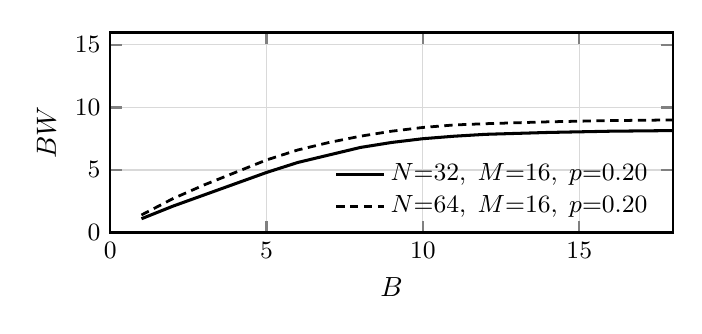
\begin{tikzpicture}
\begin{axis}[
  width=0.72\textwidth,
  height=0.34\textwidth,
  xmin=0,
  xmax=18,
  ymin=0,
  ymax=16,
  xlabel={$B$},
  ylabel={$BW$},
  axis line style={line width=0.9pt},
  tick style={line width=0.8pt},
  ticklabel style={font=\small},
  major grid style={draw=black!15},
  grid=major,
  legend style={font=\small,draw=none,fill=none,at={(0.98,0.02)},anchor=south east},
]
  % Response-shape sketch used to pick low/transition/high verification points.
  \addplot[line width=1.1pt] table[row sep=\\] {
    1 1.1\\
    2 2.1\\
    3 3.0\\
    4 3.9\\
    5 4.8\\
    6 5.6\\
    7 6.2\\
    8 6.8\\
    9 7.2\\
    10 7.5\\
    11 7.7\\
    12 7.85\\
    14 8.0\\
    16 8.1\\
    18 8.15\\
  };
  \addplot[densely dashed,line width=1.0pt] table[row sep=\\] {
    1 1.4\\
    2 2.7\\
    3 3.8\\
    4 4.8\\
    5 5.8\\
    6 6.6\\
    7 7.2\\
    8 7.7\\
    9 8.1\\
    10 8.4\\
    11 8.6\\
    12 8.7\\
    14 8.85\\
    16 8.95\\
    18 9.0\\
  };
  \addlegendentry{$N{=}32,\;M{=}16,\;p{=}0.20$}
  \addlegendentry{$N{=}64,\;M{=}16,\;p{=}0.20$}
\end{axis}
\end{tikzpicture}
\caption{Bandwidth Response Shape for Verification-Point Selection}
\label{fig:ch5-verification-shape}
\end{figure}

\section{A Synchronous Queueing Model}
\label{sec:mp-sync-queue}

The analytic model and \texttt{bws1} assume that a blocked request to module
$j$ may be reassigned randomly on reissue. To remove that assumption, a
queueing model is used in which module and bus requests are handled in
first-in, first-out order.

The queueing model structure (Figure~5.6) is still a closed queueing network.
Processors are represented by a delay server (no queueing at the processor
node). A request selects a memory module, queues for that module, then queues
for a bus, and transfer proceeds only when both resources are held. This
simultaneous resource possession is a common pattern in computer systems.

In this notation:
\begin{itemize}
\item memory modules are modeled as token-based resources (reserve/release),
\item buses are modeled as a multiserver queue.
\end{itemize}

\begin{figure}[ht]
\centering
\begin{tikzpicture}[node distance=1.2cm]
  \node[draw,circle,minimum size=0.9cm] (cpu1) {CPU};
  \node[draw,rectangle,minimum width=1.2cm,minimum height=0.8cm,right=2.2cm of cpu1] (mqueue) {M-queue};
  \node[draw,rectangle,minimum width=1.2cm,minimum height=0.8cm,right=1.8cm of mqueue] (mods) {M mods};
  \node[draw,rectangle,minimum width=1.2cm,minimum height=0.8cm,below=1.4cm of mods] (bqueue) {B-queue};
  \node[draw,rectangle,minimum width=1.2cm,minimum height=0.8cm,left=1.8cm of bqueue] (bus) {B buses};
  \node[draw,circle,minimum size=0.9cm,left=2.2cm of bus] (cpu2) {CPU};

  \draw[-{Stealth[length=3mm]},line width=0.9pt] (cpu1) -- node[above,sloped] {request} (mqueue);
  \draw[-{Stealth[length=3mm]},line width=0.9pt] (mqueue) -- (mods);
  \draw[-{Stealth[length=3mm]},line width=0.9pt] (mods) -- (bqueue);
  \draw[-{Stealth[length=3mm]},line width=0.9pt] (bqueue) -- (bus);
  \draw[-{Stealth[length=3mm]},line width=0.9pt] (bus) -- node[below,sloped] {completion} (cpu2);
  \draw[-{Stealth[length=3mm]},line width=0.9pt] (cpu2) to[bend left=20] node[left] {next cycle} (cpu1);
\end{tikzpicture}
\caption{Multiprocessor System Queueing Model Diagram}
\label{fig:ch5-queue-diagram}
\end{figure}

\paragraph{Simulation model \texttt{bws2}.}
A queueing-based model can be built by reusing parts of \texttt{bws1}
(declarations, initialization framework, and \texttt{begin cycle()}) and
replacing request/completion logic with separate module-queue and bus-queue
event routines (book Figure~5.7). In \texttt{main()}, switch dispatch is
adjusted accordingly, and \texttt{report()} can be used to obtain memory and bus
queue lengths in addition to utilizations.

Operationally, \texttt{bws2} remains synchronous. Processors with
\texttt{req[n] != 0} already have queued or active requests and are skipped in
\texttt{begin cycle()}. Module requests queue at module servers; admitted module
requests then queue at the bus server; transfer completion events mark requests
done and drive cycle-end release and scheduling logic.

\begin{figure}[ht]
\centering
\begin{minipage}{0.86\textwidth}
\begin{verbatim}
/* delta from bws1 to bws2 */
- req_module() reserves module and bus simultaneously
+ req_module() queues by module, then issues req_bus()

+ req_bus() {
+   if (busy(bus)) queue(bus); else reserve(bus);
+   schedule(END_CYCLE, 1.0, token);
+ }

- end_cycle() releases module/bus immediately
+ end_cycle() defers release until all cycle requests complete
+ and then triggers begin_cycle() for next machine cycle

+ report() now prints U(bus), U(module[j]), Q(module[j]), Q(bus)
\end{verbatim}
\end{minipage}
\caption{Changes to \texttt{bws1} for Memory and Bus Queueing}
\label{fig:ch5-bws2-delta}
\end{figure}

A key difference from \texttt{bws1} is that release operations are deferred
until all bus requests issued in the current cycle complete. Without this
deferral, resource release could trigger immediate dequeue/reschedule behavior
that invalidates cycle-level accounting.

\section{An Asynchronous Queueing Model}
\label{sec:mp-async-queue}

\texttt{bws1} and \texttt{bws2} are synchronous, fixed-cycle models. Queueing
network models are often used without strict synchronous constraints, so an
asynchronous variant is useful for comparison.

An asynchronous model (\texttt{bws3}) is obtained by simplifying \texttt{bws2}:
batching logic for cycle alignment is removed, event routines are compacted,
and processor execution intervals are generated from an exponential
distribution rather than geometric (since integer cycle counts are no longer
required).

\begin{figure}[ht]
\centering
\begin{minipage}{0.86\textwidth}
\begin{verbatim}
/* bws3 asynchronous model outline */
initialize modules[M], buses[B], processors[N]
for each processor n: schedule(ISSUE, expntl(1/p), n)

ISSUE(n):
  j = randint(1, M)
  if (module[j] and bus available) then
    reserve(module[j]); reserve(bus)
    schedule(COMPLETE, 1.0, n)
  else
    enqueue request (n,j)

COMPLETE(n):
  release resources for n
  schedule(ISSUE, expntl(1/p), n)
  dequeue waiting requests if resources become available
\end{verbatim}
\end{minipage}
\caption{Multiprocessor Simulation Model \texttt{bws3}}
\label{fig:ch5-bws3}
\end{figure}

\section{Model Results}
\label{sec:mp-results}

With the analytic model and simulation models (\texttt{bws1}, \texttt{bws2},
\texttt{bws3}), representative comparisons are shown in Table~\ref{tab:ch5-results}.

\begin{table}[ht]
\centering
\small
\begin{tabular}{rrrrrrrr}
\toprule
$N$ & $M$ & $B$ & $p$ & bwa & bws1 & bws2 & bws3 \\
\midrule
4 & 4 & 4 & 1.000 & 2.734 & 2.739 & 2.619 & 2.613 \\
4 & 4 & 2 & .500 & 1.583 & 1.668 & 1.664 & 1.665 \\
4 & 4 & 1 & .250 & .807 & .827 & .927 & .839 \\
4 & 2 & 1 & .125 & .481 & .487 & .737 & .484 \\
8 & 8 & 8 & 1.000 & 9.231 & 9.253 & 4.948 & 4.934 \\
8 & 8 & 4 & .500 & 3.273 & 3.379 & 3.334 & 3.352 \\
8 & 8 & 2 & .250 & 1.706 & 1.744 & 1.791 & 1.739 \\
8 & 4 & 2 & .250 & 1.690 & 1.711 & 1.718 & 1.709 \\
8 & 4 & 1 & .125 & .860 & .866 & .993 & .861 \\
16 & 16 & 16 & 1.000 & 10.303 & 10.305 & 9.614 & 9.586 \\
16 & 16 & 8 & .500 & 6.713 & 6.847 & 6.744 & 6.736 \\
16 & 16 & 4 & .250 & 3.553 & 3.598 & 3.601 & 3.596 \\
16 & 8 & 4 & .250 & 3.483 & 3.524 & 3.510 & 3.490 \\
16 & 8 & 2 & .125 & 1.794 & 1.794 & 1.810 & .877 \\
\bottomrule
\end{tabular}
\caption{Analytic and Simulation Model Results}
\label{tab:ch5-results}
\end{table}

In these comparisons, analytic and \texttt{bws1} bandwidths are generally close.
\texttt{bws2} and \texttt{bws3} are also close over most settings, with notable
differences for some single-bus configurations. The table supports two points:
(1) the analytic model is a useful approximation in much of the parameter
space, and (2) queueing semantics and synchrony assumptions can matter in edge
configurations.

\section{Extending the Multiprocessor System Model}
\label{sec:mp-extensions}

Natural extensions include:
\begin{itemize}
\item non-identical processors (different miss rates and execution
  distributions),
\item non-uniform/non-random memory addressing (including burst behavior),
\item variable transfer lengths (multi-cycle transfers),
\item different bus and memory service times.
\end{itemize}

All of these are straightforward to incorporate in the simulation framework
once processor/request state is explicitly represented.

\section{A CPU Modeling Project}
\label{sec:mp-cpu-project}

The chapter then introduces a project model of a pipelined CPU, intended as a
processor element that could sit inside the multiprocessor environment.
Principal elements are a four-stage instruction pipeline, a unified cache, an
instruction fetch buffer, and a data fetch buffer (Figure~5.9).

\begin{figure}[ht]
\centering
\begin{tikzpicture}[x=0.9cm,y=0.9cm]
  \node[draw,rectangle,minimum width=1.2cm,minimum height=0.8cm] (if) at (0,2.6) {Ifetch};
  \node[draw,rectangle,minimum width=1.2cm,minimum height=0.8cm] (pipeD) at (2.0,2.6) {D};
  \node[draw,rectangle,minimum width=1.2cm,minimum height=0.8cm] (pipeA) at (3.6,2.6) {A};
  \node[draw,rectangle,minimum width=1.2cm,minimum height=0.8cm] (pipeX) at (5.2,2.6) {X};
  \node[draw,rectangle,minimum width=1.2cm,minimum height=0.8cm] (pipeW) at (6.8,2.6) {W};
  \node[draw,rectangle,minimum width=2.0cm,minimum height=0.8cm] (cache) at (3.6,1.1) {Cache};
  \node[draw,rectangle,minimum width=1.2cm,minimum height=0.8cm] (df) at (6.8,1.1) {Dfetch};
  \draw[-{Stealth[length=3mm]},line width=0.9pt] (if) -- (pipeD);
  \draw[-{Stealth[length=3mm]},line width=0.9pt] (pipeD) -- (pipeA);
  \draw[-{Stealth[length=3mm]},line width=0.9pt] (pipeA) -- (pipeX);
  \draw[-{Stealth[length=3mm]},line width=0.9pt] (pipeX) -- (pipeW);
  \draw[-{Stealth[length=3mm]},line width=0.9pt] (pipeA) -- (cache);
  \draw[-{Stealth[length=3mm]},line width=0.9pt] (cache) -- (df);
  \draw[-{Stealth[length=3mm]},line width=0.9pt] (df) -- (pipeX);
\end{tikzpicture}
\caption{Major CPU Elements}
\label{fig:ch5-cpu-elements}
\end{figure}

Pipeline stages are fetch/decode (D), address generation (A), execute (X), and
write-back (W). At least one cycle is spent in each stage, so minimum
instruction latency is four cycles, while peak throughput is one instruction
per cycle due to overlap.

Branch and fetch/store behavior, cache arbitration, and multi-cycle execute
operations introduce holes and blocking effects in the completion stream, which
makes this a useful project for studying pipeline-control and memory-system
interaction under simulation.

Figure~5.10 in the original text illustrates representative pipeline sequences
and delay patterns for instruction classes:
\begin{itemize}
\item \textbf{FS}: load/store/non-taken branch instructions (issue cache request
  in first A cycle),
\item \textbf{BR}: taken branch instructions (issue target fetch in first A
  cycle),
\item \textbf{ALU}: arithmetic/logic instructions (may require multiple X
  cycles).
\end{itemize}

\begin{figure}[ht]
\centering
\begin{minipage}{0.86\textwidth}
\centering
\small
\begin{tabular}{l|cccccccc}
sequence & 1 & 2 & 3 & 4 & 5 & 6 & 7 & 8 \\ hline
(a) ALU  & D & A & X & W & D & A & X & W \\ 
(b) FS   & D & A & C & W & O & D & A & W \\ 
(c) BR   & D & A & B & O & O & D & A & W \\ 
(d) mix  & D & A & X & X & W & D & A & W \\ 
(e) mix  & D & A & B & O & D & A & X & W \\ 
\end{tabular}
\par\vspace{0.4em}
\footnotesize O = hole, C = cache arbitration delay, B = taken branch delay
\end{minipage}
\caption{Pipeline Sequence Examples}
\label{fig:ch5-pipeline-examples}
\end{figure}

In these sequences, \texttt{O} marks holes propagating through the pipeline and
\texttt{@} marks a delay cycle (a cycle in which no instruction completes).
Important effects shown in the examples:
\begin{itemize}
\item multi-X-cycle ALU instructions interlock following instructions;
\item FS requests can delay sequential instruction fetches and create holes;
\item taken branches can create multi-cycle holes due to target-fetch latency;
\item some holes are masked by other delays (e.g., long X-stage occupancy).
\end{itemize}

\paragraph{Workload description.}
Design evaluations for this project use the following instruction mix:

\begin{table}[ht]
\centering
\begin{tabular}{lr}
\toprule
Instruction type & Proportion \\
\midrule
BR  & 0.1437 \\
FS  & 0.4002 \\
ALU & 0.4561 \\
\midrule
Total & 1.0000 \\
\bottomrule
\end{tabular}
\caption{CPU Project Instruction Mix}
\label{tab:ch5-instr-mix}
\end{table}

FS instructions are approximately 49.5\% fetches, 17.5\% stores, and 33.0\%
non-taken branches. BR and FS instructions always have single-cycle X stages.
ALU instructions use a variable number of X cycles:

\begin{table}[ht]
\centering
\begin{tabular}{lr}
\toprule
ALU X cycles & Proportion of ALU instructions \\
\midrule
1  & 0.40 \\
2  & 0.40 \\
4  & 0.10 \\
8  & 0.07 \\
16 & 0.03 \\
\midrule
Total & 1.00 \\
\bottomrule
\end{tabular}
\caption{ALU Operation-Time Mix}
\label{tab:ch5-alu-mix}
\end{table}

Inter-branch headways (instructions between taken branches) are generated from
the distribution used earlier in Chapter 1. BR instructions terminate a
headway; other instructions in a headway are assigned independently as FS or
ALU according to the proportions above.

\paragraph{Building and validating the model.}
A compact smpl model is feasible (the original notes indicate under 100 lines
of C excluding debug instrumentation). A practical implementation strategy is to
compute stage transitions backward (W$\rightarrow$A) per cycle rather than
forward.

Validation in this project is primarily trace-based (in the absence of direct
analytic baselines for all behaviors). A useful cycle trace includes D/A/X/W
stage contents and key state such as Ifetch-buffer occupancy and sequential
fetch/branch flags.

\paragraph{Pipeline design analyses.}
Primary performance metric: mean instruction execution time per instruction,
$I$ cycles/instruction. If cycle time is $C$ microseconds, throughput in MIPS is
$(IC)^{-1}$. Also collect mean X-stage cycles per instruction, $E$; branch/Ifetch
delay contribution is then $D = I - E$.

The base case is Ifetch-buffer capacity of one instruction. Alternatives to
evaluate relative to this baseline:
\begin{enumerate}
\item increase Ifetch-buffer capacity to 2, 3, or 4 instructions;
\item widen cache$\rightarrow$Ifetch path so sequential/target fetch can return two
  instructions per cache access (with and without enforced branch-target
  alignment);
\item delayed-branch architecture variant where the sequential instruction
  following a branch always executes (assume useful work 70\%, NOP 30\%);
\item repeat evaluations assuming multi-cycle ALU execution times are reduced by
  50\% in a future implementation.
\end{enumerate}
